%% LyX 2.1.4 created this file.  For more info, see http://www.lyx.org/.
%% Do not edit unless you really know what you are doing.
\documentclass[english]{article}
\usepackage[T1]{fontenc}
\usepackage[latin9]{inputenc}
\usepackage{amsmath}
\usepackage{amssymb}
\usepackage{graphicx}
\usepackage{babel}
\begin{document}

\section{Derivation}

\begin{figure}[h]
\begin{centering}
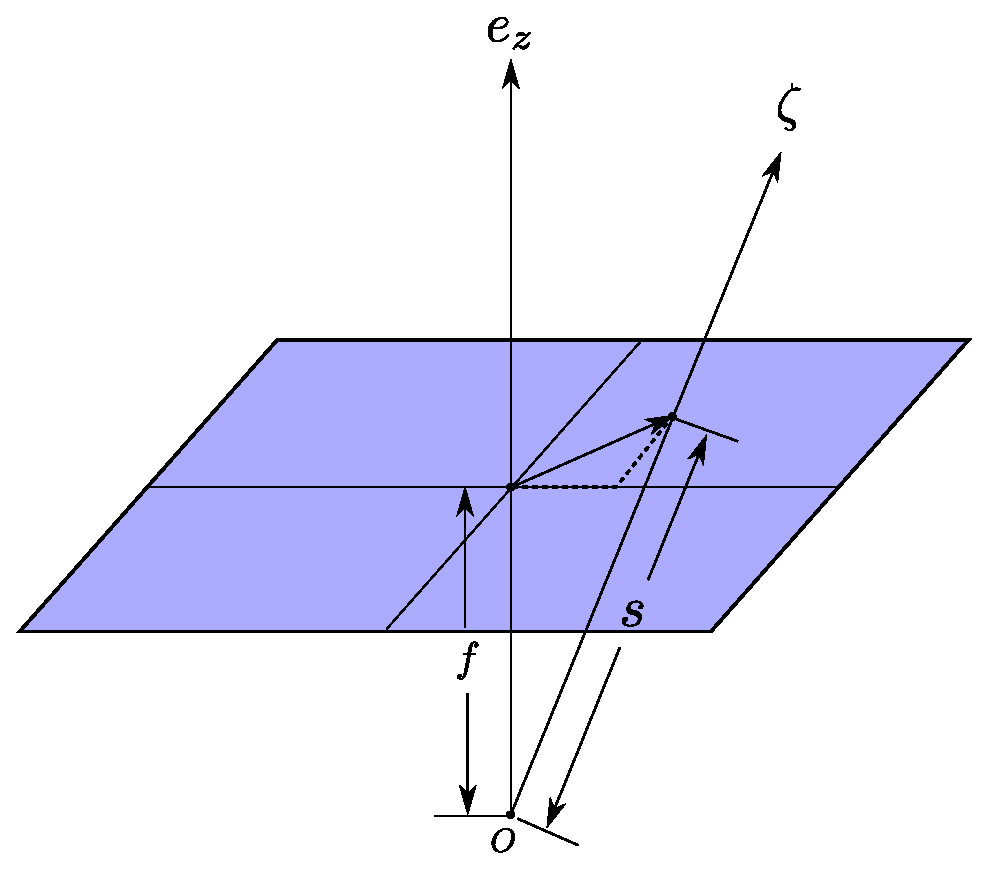
\includegraphics[width=0.8\textwidth]{figures/pixel_geometry}\\
\label{fig:pixel_geometry}
\par\end{centering}

\caption{Camera Pixel and feature vector geometry}
\end{figure}


\[
\begin{aligned}e_{z}\cdot\left(-fe_{z}+s\zeta\right) & =0\\
\left(e_{z}\cdot s\zeta\right)-\left(e_{z}\cdot fe_{z}\right) & =0\\
s\left(e_{z}\cdot\zeta\right) & =\left(e_{z}\cdot fe_{z}\right)\\
s & =\frac{e_{z}\cdot fe_{z}}{e_{z}\dot{\zeta}}\\
 & =\frac{f}{e_{z}\zeta}\\
 & =\frac{f}{e_{z}^{\top}\zeta}
\end{aligned}
\]


\[
\begin{aligned}\lambda & =\left[\begin{array}{ccc}
1 & 0 & 0\\
0 & 1 & 0
\end{array}\right]s\zeta\\
 & =I_{2\times3}s\zeta\\
 & =I_{2\times3}\frac{f}{e_{z}\zeta}\zeta
\end{aligned}
\]



\section{Helpful Identity}

\[
\boldsymbol{\zeta}=R\left(q_{c}^{\zeta}\right)^{\top}\boldsymbol{e}_{z}\in\mathcal{S}^{2}\subset\mathbb{R}^{3}
\]


\[
T_{\zeta}=R\left(q_{c}^{\zeta}\right)^{\top}\left[\begin{array}{cc}
\boldsymbol{e}_{x} & \boldsymbol{e}_{y}\end{array}\right]\in\mathbb{R}^{3\times2}
\]


\[
\begin{aligned}\frac{d}{dq_{\zeta}^{c}}\zeta^{c} & =\frac{d}{dq_{\zeta}^{c}}\left(R\left(q_{\zeta}^{c}\right)^{\top}e_{z}\right)\\
 & =\left\lfloor \zeta\right\rfloor T_{\zeta}
\end{aligned}
\]



\section{Jacobian}

You have to use the quotient rule to deal with the $\zeta$ on the
bottom, and the chain rule to deal with the $\zeta$ multiplied. Something
is still wrong though, because the sizes don't match up for the first
term.

\[
\begin{aligned}\frac{\partial\lambda}{\partial q_{c}^{\zeta}} & =\frac{\partial}{\partial q_{c}^{\zeta}}\left(I_{2\times3}\frac{f}{e_{z}^{\top}\zeta}\zeta\right)\in\mathbb{R}^{2\times2}\\
 & =I_{2\times3}\left(\frac{-fe_{z}^{\top}\left\lfloor \zeta\right\rfloor T_{\zeta}}{\left(e_{z}^{\top}\zeta\right)^{2}}\zeta+\frac{f}{e_{z}^{\top}\zeta}\zeta\left\lfloor \zeta\right\rfloor T_{\zeta}\right)\\
 & =I_{2\times3}f\frac{\partial}{\partial q_{c}^{\zeta}}\left(\frac{\zeta}{e_{z}^{\top}\zeta}\right)\in\mathbb{R}^{2\times2}\\
 & =I_{2\times3}f\left(\frac{\frac{\partial}{\partial q_{c}^{\zeta}}\left(\zeta\right)}{e_{z}^{\top}\zeta}+\frac{\partial}{\partial q_{c}^{\zeta}}\left(\frac{1}{e_{z}^{\top}\zeta}\right)\zeta\right)
\end{aligned}
\]

\end{document}
